In questo esperimento si vuole controllare un LED RGB tramite l'azionamento di un potenziometro. Per questo esperimento sono stati utilizzati i seguenti componenti:
\begin{itemize}
    \item Resistenze $R_R,R_G,R_B$ da determinare, $0.25$ W. 
    \item LED RGB SMD, codice \textit{ASMB-MTB0-0A3A2}, Avago
    \item 3 transisor NPN, codice \textit{P2N2222AG}, ON Semiconductor
    \item Potenziometro lineare $R_{var}:10\text{ k}\Omega$
    \item Scheda Arduino DUE
    \item Interruttore
\end{itemize}
Il circuito riportato in Figura \ref{fig:Circuit2} è alimentato mediante porta USB del PC, la quale eroga circa $(\sim 5 V)$
\begin{figure}[H]
    \centering
    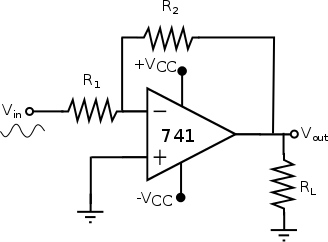
\includegraphics[width=0.4\linewidth]{images/Circuit2.png}
    \caption{Schema circuito}
    \label{fig:Circuit2}
\end{figure}
\noindent Il potenziometro è collegato al pin analogico \textbf{A0}, mentre i tre led sono collegati ai pin digitali \textbf{12,11,10}.
\subsection{Dimensionamento circuito e analisi - prelab}
La massima corrente erogabile da un pin digitale di Arduino DUE è 
\begin{equation*}
    I_{OUT.MAX}=3\text{ mA}
\end{equation*}
La tensione nominale dei tre diodi LED utilizzati, ricavata dal datasheet vale
\begin{equation*}
    V_{ON.R}=2.1\text{ V}\quad V_{ON.G}=3.1\text{ V}\quad V_{ON.B}=3.1\text{ V}
\end{equation*}
Si vuole ora dimensionare le resistenze di base dei transistor in modo che la corrente erogata dai pin digitali sia pari a $2.5\text{ mA}$, si considera per i calcoli che il transistor abbia $V_{BE}=0.7\text{ V}$
\begin{equation*}
    R_{B.R}=1\text{ k$\Omega$}\quad R_{B.G}=1\text{ k$\Omega$}\quad R_{B.B}=1\text{ k$\Omega$}
\end{equation*}
Nell'ipotesi che i transistor funzionino in saturazione, si dimensionano le resistenze di collettore dei tre BJT in modo che la corrente sui LED sia pari a $7 \text{ mA}$.
\begin{equation*}
    R_{C.R}=180\text{ $\Omega$}\quad R_{C.G}=33\text{ $\Omega$}\quad R_{C.B}=33\text{ $\Omega$}
\end{equation*}
\subsection{Codice e misure - 1}
Dopo il montaggio del circuito si è scritto un semplice programma che accende i tre LED in DC. Il codice è molto semplice e non richiede nemmeno l'uso del \texttt{void loop()}.
\begin{lstlisting}[frame=single, language=Arduino]
const int RedLedPin = 12;     // Red LED to digital pin 12
const int GreenLedPin = 11;   // Green LED to digital pin 11
const int BlueLedPin = 10;    // Blue LED to digital pin 10

void setup(){
    pinMode(RedLedPin, OUTPUT);     // Set Red LED pin as output
    pinMode(GreenLedPin, OUTPUT);   // Set Green LED pin as output
    pinMode(BlueLedPin, OUTPUT);    // Set Blue LED pin as output
    
    digitalWrite(RedLedPin, HIGH);  // Turn on Red LED
    digitalWrite(GreenLedPin, HIGH);// Turn on Green LED
    digitalWrite(BlueLedPin, HIGH); // Turn on Blue LED
}

void loop(){} // The void loop is empty
\end{lstlisting}
In queste condizioni sono state effettuate alcune misure.\\ 
Dapprima è stata misurata la caduta di tensione base-emettitore dei tre transistor:
\begin{equation*}
    V_{BE.R}=0.742\text{ V}\quad V_{BE.G}=0.761\text{ V}\quad V_{BE.B}=0.761\text{ V}
\end{equation*}
Si è misurata anche la corrente erogata dalle uscite digitali
\begin{equation*}
    I_{pin10}=2.46\text{ mA}\quad I_{pin11}=2.47\text{ mA}\quad V_{pin12}=2.1\text{ mA}
\end{equation*}
La tensione di funzionamento misurata dei tre LED è
\begin{equation*}
    V_{ON.R}=1.99\text{ V}\quad V_{ON.G}=2.876\text{ V}\quad V_{ON.B}=2.932\text{ V}
\end{equation*}
Si nota che questi risultati non sono esattamente quelli del datasheet !!!!!\\
Infine si misura la corrente che scorre sui tre LED
\begin{equation*}
    I_{R}=6.97\text{ mA}\quad V_{G}=14.63\text{ mA}\quad V_{B}=12.71\text{ mA}
\end{equation*}
Qual è il motivo per cui questi valori di corrente differiscono da quello scelto in fase di progetto (7 mA)?
(non abbiamo preso i valori di resistenza calcolati, bensì i più vicini in laboratorio) !!!!!
\subsection{Codice - 2}
L’ingresso analogico \textbf{A0}, a seconda della posizione del potenziometro $R_{var}$, legge valori compresi tra 0 e 1023. Si vuole  definire un algoritmo che – al ruotare del potenziometro – cambi la combinazione di colori sul LED RGB in maniera graduale. La modalità con cui cambiano i colori è espressa dalla Figura \ref{fig:RGBScale}
\begin{figure}[H]
    \centering
    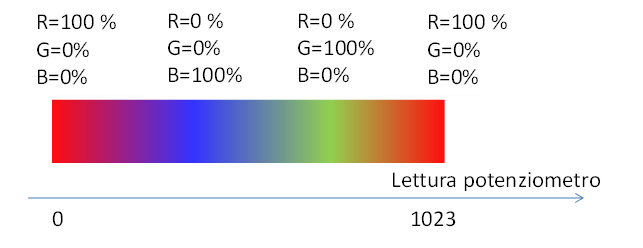
\includegraphics[width=0.8\linewidth]{images/RGBScale.png}
    \caption{Scala RGB del potenziometro}
    \label{fig:RGBScale}
\end{figure}
Abbiamo diviso la scala RGB in tre zone: da 0 a 341, da 342 a 682 e da 683 a 1023. In ciascuna di queste zone abbiamo fatto variare il valore della componente di colore sulla base del grafico in Figura \ref{fig:RGBScale} facendo variare opportunamente il valore del canale del LED da 0 a 255. Si riporta il codice dell'algoritmo implementato
\begin{lstlisting}[frame=single, language=Arduino]
const int RedLedPin = 12;     // Red LED to digital pin 12
const int GreenLedPin = 11;   // Green LED to digital pin 11
const int BlueLedPin = 10;    // Blue LED to digital pin 10

const int PotPin = A0;  // Pot. for RGB control to analog pin A0

const float K = 0.7478; // approx 255/341

int RedLedBright = 0;   // Red LED brightness
int GreenLedBright = 0; // Green LED brightness
int BlueLedBright = 0;  // Blue LED brightness

void setup(){
    pinMode(RedLedPin, OUTPUT);     // Set Red LED pin as output
    pinMode(GreenLedPin, OUTPUT);   // Set Green LED pin as output
    pinMode(BlueLedPin, OUTPUT);    // Set Blue LED pin as output
}
\end{lstlisting}
\clearpage
\begin{lstlisting}[frame=single, language=Arduino]
void loop(){
    int PotValue = analogRead(PotPin);  // Read potentiometer value

    if(PotValue == 0){
        RedLedBright = 255;
        GreenLedBright = 0;
        BlueLedBright = 0;
    } else if(PotValue < 341){
        RedLedBright = 255 - PotValue*K;
        GreenLedBright = 0;
        BlueLedBright = PotValue*K;
    } else if(PotValue < 682){
        RedLedBright = 0;
        GreenLedBright = PotValue*K - 255;
        BlueLedBright = 510 - PotValue*K;
    } else if(PotValue < 1023){
        RedLedBright = PotValue*K - 510;
        GreenLedBright = 765 - PotValue*K;
        BlueLedBright = 0;
    } else {
        RedLedBright = 255;
        GreenLedBright = 0;
        BlueLedBright = 0;
    }

    // Set LED brightness
    analogWrite(RedLedPin, RedLedBright); 
    analogWrite(GreenLedPin, GreenLedBright);
    analogWrite(BlueLedPin, BlueLedBright);   
}
\end{lstlisting}
L'aggiunta della lettura avviene aggiungendo la seguente riga nel \texttt{void setup()} che serve per inizializzare la connessione seriale
\begin{lstlisting}[frame=single, language=Arduino]
void setup(){   [...]
    Serial.begin(9600);
}
\end{lstlisting}
E la seguente riga nel \texttt{void loop()} per stampare sul serial monitor l'intensità (da 0 a 255) del segnale sul LED rosso, verde e blu.
\begin{lstlisting}[frame=single, language=Arduino]
Serial.println("RED: %d GREEN: %d BLUE: %d", RedLedBright, GreenLedBright, BlueLedBright); 
\end{lstlisting}
E' possibile apprezzare il funzionamento del circuito dal video al \href{https://mediaspace.unipd.it/media/Esperimento+2/1_y2jgm47p}{seguente link}
\subsection{Codice - 3}
Nell'ultima parte è stato connesso un secondo potenziometro al pin analogico \textbf{A1} e il programma è stato modificato in modo che questo secondo potenziometro permetta di regolare l’intensità luminosa complessiva della luce emessa dal LED RGB\\\\
Si riporta in seguito le modifiche apportate al codice
\begin{lstlisting}[frame=single, language=Arduino]
const int LuxPin = A2;  // Pot. for brightness control to analog pin A0 

int TotBright = 0;

/*
    ************* VOID SETUP *************
*/

void loop(){
    int PotValue = analogRead(PotPin);  // Read potentiometer value
    
    /*
        ************* RGB ALGORITHM *************
    */
    
    int LuxValue = analogRead(LuxPin);  // Read potentiometer value
    TotBright = map(LuxValue, 0, 1023, 0, 100);

    RedLedBright *= TotBright /100;
    GreenLedBright *= TotBright /100;
    BlueLedBright *= TotBright /100;

    // Set LED brightness
    analogWrite(RedLedPin, RedLedBright); 
    analogWrite(GreenLedPin, GreenLedBright);
    analogWrite(BlueLedPin, BlueLedBright);

    Serial.println("RED: %d GREEN: %d BLUE: %d", RedLedBright, GreenLedBright, BlueLedBright);    
}
\end{lstlisting}
E' possibile apprezzare il funzionamento del circuito dal video al \href{https://mediaspace.unipd.it/media/Esperimento+2.1/1_ewlxzlyv}{seguente link}